\section{Methods and technical infrastructure}\label{sec:methods}

This section describes the ACI support that made this workshop possible, and
highlights reusable and shareable patterns to build on for future work. We will
begin with a rough guide to the steps required to replicate this style of
bootcamp elsewhere, and then cover more details as to the specific hardware and
software implementations.

For instructors interested in hosting a similar event at their institution, the
following steps should be taken:

\begin{enumerate}
\item Contact your local XSEDE Campus Champion
\item Decide on the resources needed (e.g. number of nodes, GPUs, etc)
\item Make a plan for spin-down of cloud instances after the class
\item Apply for an XSEDE Education Allocation for Jetstream
\item Install Docker for Mac or Docker for Windows on laptop
\item Build docker container based on the jupyter/datascience-notebook \footnote{https://github.com/jupyter/docker-stacks/tree/master/datascience-notebook}
\item Instructors create course materials on a shared github repo
\item Test instructor's Jupyter notebooks in Docker on laptop
\item Provision virtual machines (VMs) on Jetstream
\item Deploy custom docker container on Jetstream VMs
\item Send IP addresses for each machine to students (one per student)
\item Connect from your browser to Jupyter notebooks running on Jetstream IP address
\item Run the bootcamp
\item Assist students in migrating work onto their own machines
\end{enumerate}

All Jupyter notebook content for the course is available at:\\
\indent\indent\url{https://github.com/choldgraf/UCSF-Data_Driven_Neuro}

All build and deploy scripts are available at:\\
\indent\indent\url{https://github.com/aculich/UCSF-Data_Driven_Neuro-deploy}

\begin{figure}[h]
\centering
% See also: docker-jetstream-process.xml
% which is generated using: https://www.draw.io/
\includegraphics[width=0.5\textwidth]{docker-jetstream-process.png}
\caption{Overview building Docker container and deploying to Jetstream for bootcamp}
\end{figure}

\subsection{Computational resources and the XSEDE Jetstream cloud}

The Jetstream~\cite{Stewart2015Jetstream} cloud platform
(\url{http://jetstream-cloud.org/}) provided the computational resources for the
workshop. Jetstream's core capabilities include the ability to create
interactive Virtual Machines (VMs), access to remote desktops through a web
browser, and publishing VMs with a Digital Object Identifier (DOI). Jetstream is
attractive because it provides researchers a simple web-based
interface\cite{NiravCyberinfra2016} to launch, provision, manage, build, and
share customized virtual machines that include complete software dependencies
for running complex applications, whereas HPC environments traditionally do not
provide full administrative (root) access and are often not as flexible as
cloud-based virtual machines.

\begin{figure}[h]
\centering
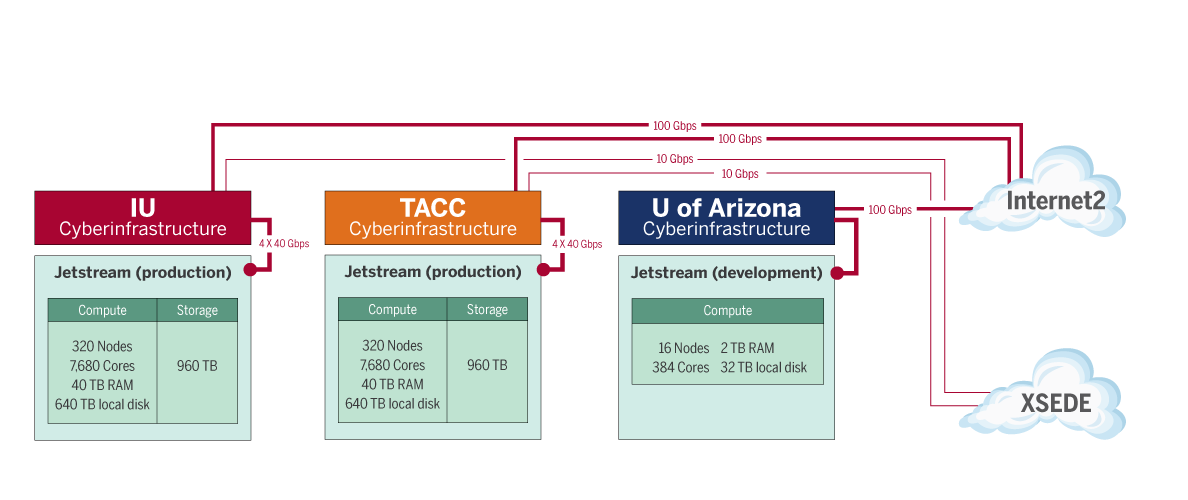
\includegraphics[width=0.5\textwidth]{jetstream-0.png}
\caption{XSEDE Jetstream cloud production infrastructure provided by Indiana University (IU) and Texas Advanced Computing Center (TACC). Taken from \url{http://jetstream-cloud.org/technology.php}}
\end{figure}

Access to Jetstream is available to researchers at no cost through the
NSF-funded XSEDE\footnote{https://www.xsede.org/} (Extreme Science and
Engineering Discovery Environment) project~\cite{Towns2014XSEDE}. This
offers access to a plethora of supercomputers as well as high-end
visualization and data-analysis resources across the
country in order to address increasingly diverse scientific and
engineering challenges.

To obtain access, a qualified Principal Investigator writes a resource
justification and submits an allocation request. To help speed up the
process of choosing and obtaining access to the resource, many campuses
have local XSEDE Campus Champions who can facilitate quick access and
help prepare an allocation request.

For the neuroimaging workshop, the local Campus Champion worked with Berkeley
Institute for Data Science (BIDS) and eScience Institute data scientists to
prepare an Education Allocation request. Below are some key excerpts from the
1-page allocation request \footnote{\url{https://portal.xsede.org/documents/10308/29438/Jetstream+Education+Allocation+request+-+Sample/28517ffe-79fa-4e3f-98c9-b64f126a1e6b}},
which you can read in full from the list of example allocation requests:

\begin{itemize}
\item 50 Virtual Machines running simultaneously \\(40 students + 5 instructors +
test/spare/debug VMs)
\item Each VM will need to be a: Jetstream m1.medium VM \\(6 vCPUs, 16GB RAM, 60GB
  Storage)
\item Each VM will need an external IP address so students can connect remotely
  with a web browser to a Jupyter Notebook running on the machine
\item We are requesting 10,000SUs in total.
\end{itemize}

An SU is a Service Unit. The maximum number of SUs for an Education Allocation
on Jetstream is 50,000SUs, however after we calculated the total resources we
needed for the course, we determined that 10,000SUs would be sufficient to
conduct the course, as well as allow students to run VMs for a short time
following the event. The SU cost per hour for each VM can be determined at the
Jetstream General Virtual Machine Configurations page\footnote{\url{http://jetstream-cloud.org/general-vms.php}}.
At the time of the workshop the m1.medium VM noted above cost 6 SUs per hour.

The technology we used to deploy the workshop in addition to the Jetstream cloud
platform includes Docker, Dockerhub, and the datascience-notebook docker-stacks\footnote{\url{https://github.com/jupyter/docker-stacks/}}
maintained by the Jupyter project.

\subsection{Development and environment control with Docker}

Each of the instructors initially used their own laptops to develop Jupyter
Notebook-based tutorials on computer vision and machine learning for
neuroscience, using state-of-the-art deep learning methods.

Research IT staff worked with BIDS and eScience data scientists to build a
customized container from the Jupyter project's datascience-notebook image. This
provides a pre-configured Jupyter Notebook 4.3.x; Conda Python 3.x and Python
2.7.x environments; and several common libraries including: pandas
\cite{mckinney-proc-scipy-2010}, matplotlib \cite{hunter2007matplotlib}, scipy
\cite{scipy}, seaborn \cite{michael_waskom_2014_12710}, scikit-learn
\cite{Pedregosa2012-dm}, and scikit-image \cite{van2014scikit}. Additional
neuroscience-specific packages were included such as Dipy for diffusion magnetic
resonance imaging (dMRI) analysis \cite{Garyfallidis2014FrontNeuroinf}.

This customized container ensured that all the students had an identical
environment on the day of the workshop, including all required software
dependencies. The container made it possible for participants to easily run the
software without installing each of the components, often a lengthy and
error-prone process at the start of many workshops. The container can also be
used to tag version of the environment, such that the software is preserved
for future use. Months or years from now it will be possible to re-run the
notebooks again, even if external software packages and dependencies have
changed.

The container image was pushed to Docker hub (\url{https://hub.docker.com/}),
which provides a centralized resource for container image discovery,
distribution and change management, user and team collaboration, and workflow
automation. Once a Docker image is on Docker hub, it can be downloaded and run
with a single command. At a high-level the process is:

\begin{enumerate}
  \item On a laptop, create a Dockerfile that:
  \begin{itemize}
    \item derives \texttt{FROM jupyter/datascience-notebook}
    \item installs workshop-specific software packages
    \item pin packages with explicit versions defined
  \end{itemize}
  \item Build docker image
  \item Run docker image as container
  \item Test Jupyter notebooks running inside container
  \item Push docker image to DockerHub
\end{enumerate}


\subsection{Putting it together}

On the day of the workshop, the 50 Jetstream virtual machines (VMs) were
deployed by hand using Jetstream's Atmosphere\cite{NiravCyberinfra2016} web interface
(\url{http://www.cyverse.org/atmosphere}). While it is possible to create
scripts for a fully automated deployment using the low-level OpenStack API that
Jetstream is built on, we decided that the additional complexity was not
desirable. Using the Atmosphere web interface is a quick and simple 6-step
process that allowed us to manually start the deployment of all 50 instances in
just a few minutes. At a high-level the process is:

\begin{enumerate}
\item Select the pre-defined VM image: \\Ubuntu 14.04.3 Development GUI
\item Choose instance size: m1.medium VM \\(6 vCPUs, 16GB RAM, 60GB
  Storage)
\item Click ``Advanced Options''
\item Select deployment script from github URL for the workshop
\item Click ``Continue to Launch''
\item Click ``Launch Instance''
\end{enumerate}

\begin{figure}[h]
\centering
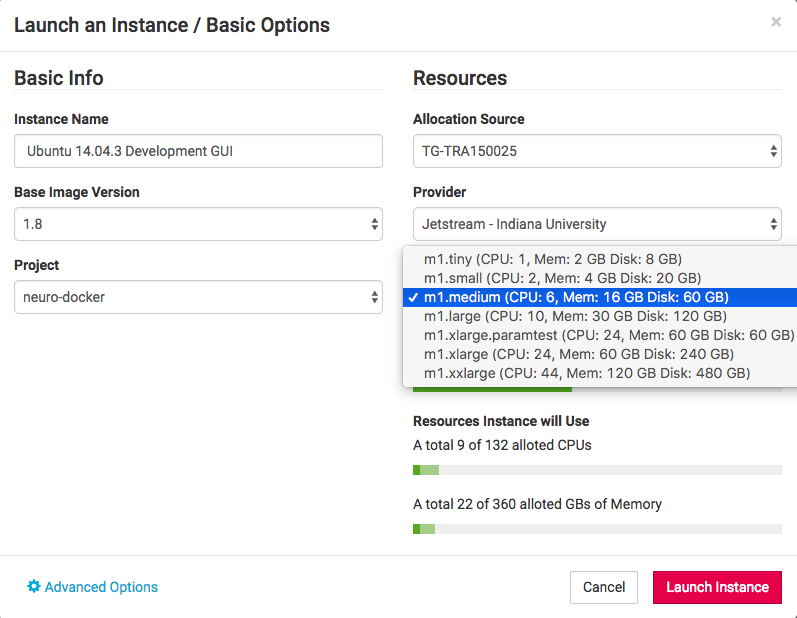
\includegraphics[width=0.5\textwidth]{jetstream-launch-instance.png}
\caption{Screenshot of configuring a virtual machine (VM) to launch on Jetstream}
\end{figure}

The deployment script from github URL for the workshop is a simple bash script
that will be run when the VM starts that does the following:

\begin{enumerate}
\item Install Docker on the Jetstream VM
\item Pull the workshop docker image from DockerHub
\item Download all the data needed for the workshop examples
\item start the Docker container running the Jupyter notebook, password-protected on a standard web port (80/443)
\end{enumerate}

After the workshop the participants were allowed to continue accessing their
notebook on the Jetstream platform for a limited time using the Education
Allocation for the workshop. After the allocation expired, each individual could
either:

\begin{itemize}

\item install Docker for Mac or Docker for Windows to download and run the
      container on their own laptop
\item apply for their own Startup and Research Allocations on XSEDE Jetstream

\end{itemize}

\subsubsection{Considerations for security and privacy}

It is worth noting a few issues related to networking and security that must be
addressed for any scenario involving remote computing (whether in a cloud
computing environment or traditional server environment).

When running Jupyter Notebooks on a laptop, they typically listen on network
port 8888 and a user connects via their web browser to
\url{http://localhost:8888}. In this configuration, the port is not accessible
to a remote attacker. In a server environment, remote access is a key
feature, so it requires running the Jupyter notebook in a secure mode requiring
a token or a password. Thankfully, the Jupyter team has configured the
docker-stacks to run in a secure mode by default.

For the workshop we chose a single password to deploy to each of the Jupyter VM
instances and wrote the password on the whiteboard for participants. We also
copied the IP address of each machine into a Google spreadsheet, and assigned it
to each of the participants. Alternative solutions to this include using a link
shortening service such as \url{http://bit.ly} to generate a URL out of student
names.
